\documentclass[10pt]{article}

\usepackage{times}
\usepackage{mathptmx}  
\usepackage{spverbatim}
\usepackage{fixltx2e}
\usepackage[utf8]{inputenc}
\usepackage{graphicx}
\usepackage{sidecap}
\usepackage{fancyhdr}
\usepackage{amssymb,amsmath}
\usepackage[swedish]{babel}
\usepackage[margin=1.5in]{geometry}
\usepackage{abstract}
\usepackage[parfill]{parskip}
\usepackage{tocloft}
\usepackage{adjustbox}
\usepackage{textcomp}
\usepackage[T1]{fontenc}
\usepackage{listings}
\usepackage{xcolor,colortbl}
\usepackage{hyperref}
\usepackage{mcode}
\usepackage{a4wide}
\usepackage{caption}
\usepackage{epstopdf}

\begin{document}

\appendix
\pagestyle{empty}
\newgeometry{left=2cm,right=2cm,bottom=2cm,top=2cm}
\section{Filtrerade signaler}

\begin{figure}[htp]
  \begin{center}
  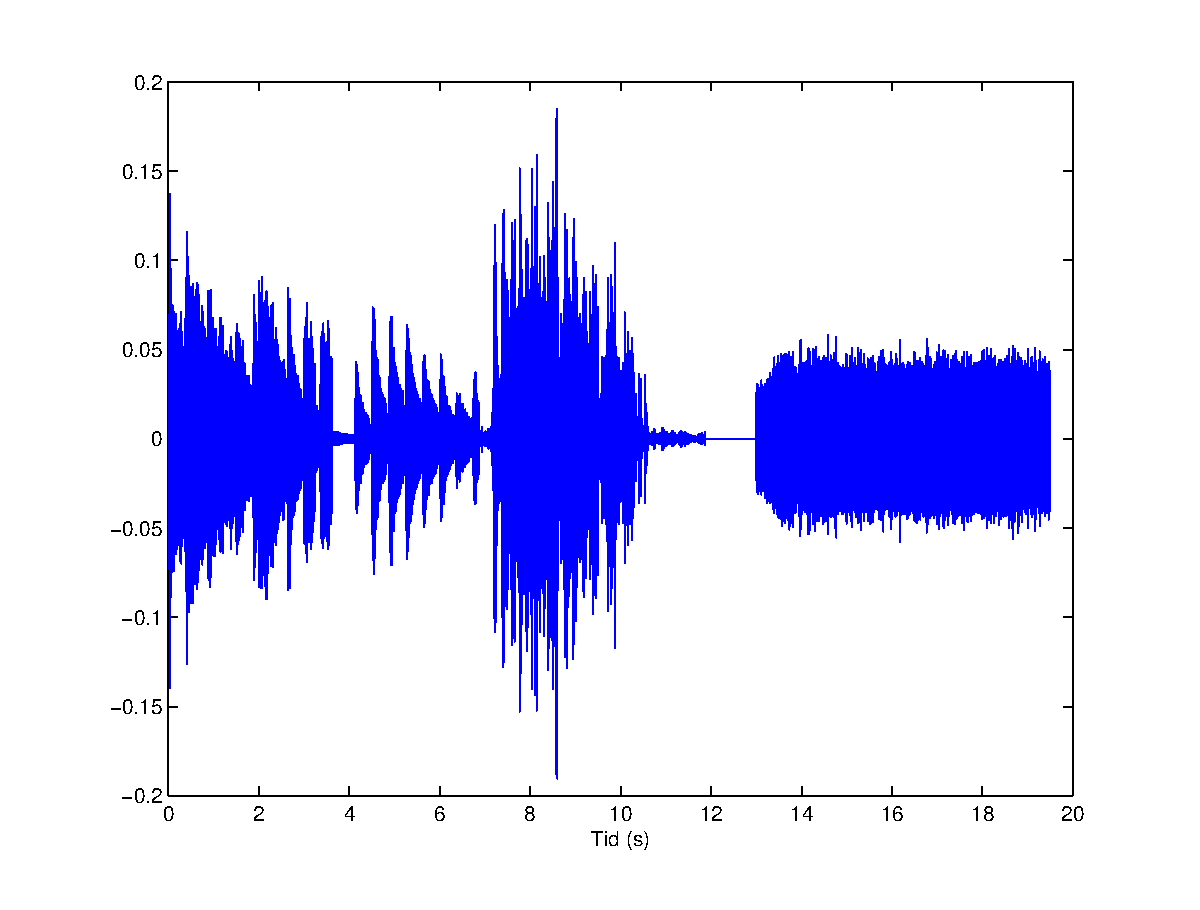
\includegraphics[keepaspectratio=true,width=\linewidth]{topp1_filter.eps}  %skala och filnamn. 
  \end{center}
  \caption{Frekvenstopp 1 filtrerad} %figurtext.
  \label{fig:topp1_filter}
\end{figure}

\begin{figure}[htp]
  \begin{center}
  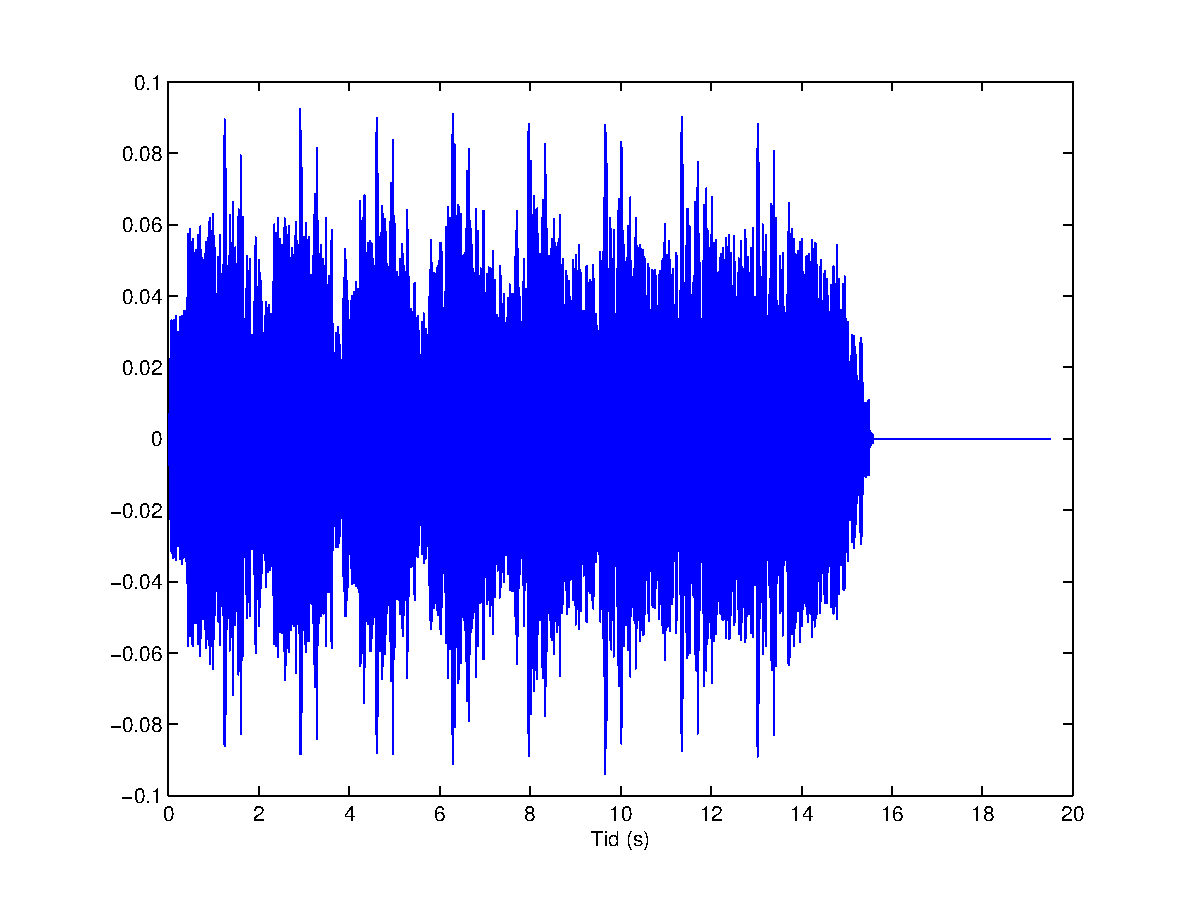
\includegraphics[keepaspectratio=true,width=\linewidth]{topp2_filter.eps}  %skala och filnamn. 
  \end{center}
  \caption{Frekvenstopp 2 filtrerad} %figurtext.
  \label{fig:topp2_filter}
\end{figure}

\begin{figure}[htp]
  \begin{center}
  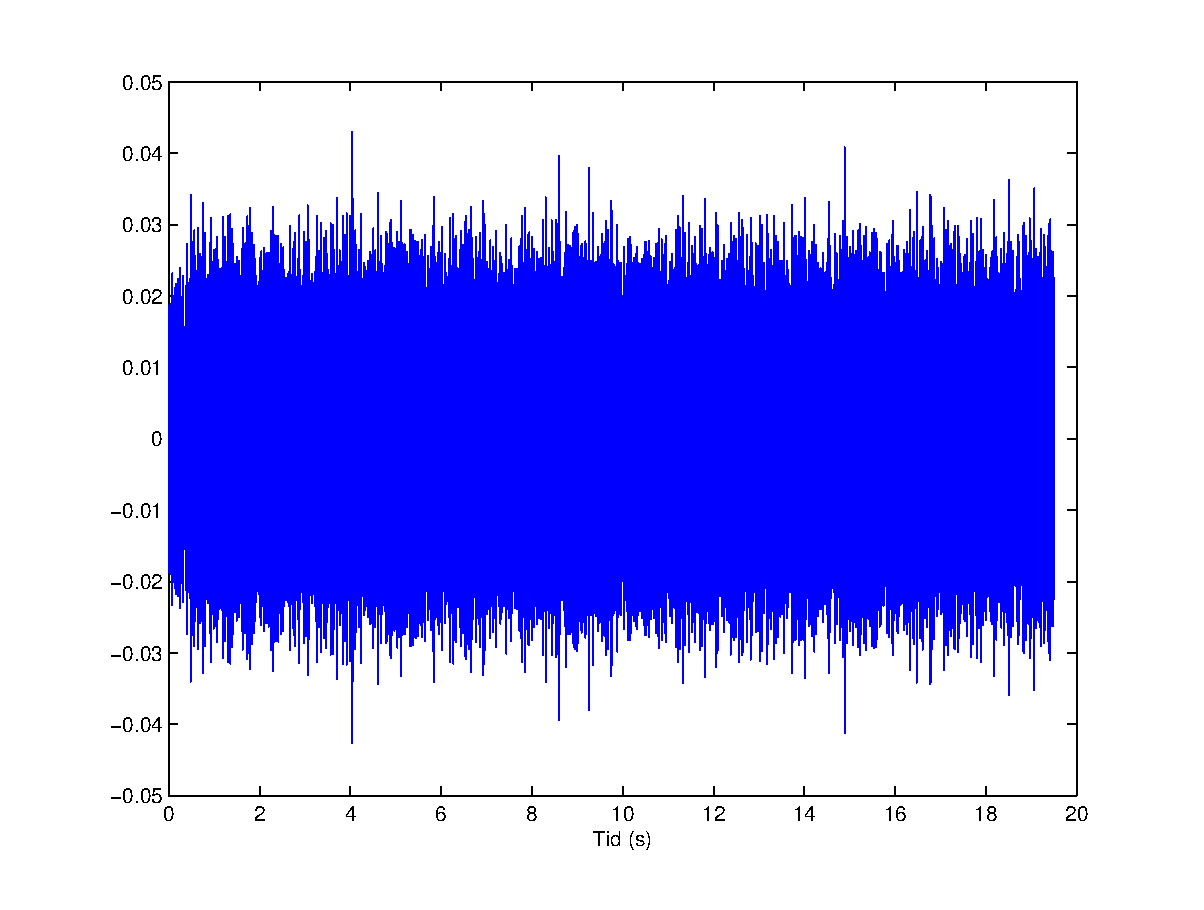
\includegraphics[keepaspectratio=true,width=\linewidth]{topp3_filter.eps}  %skala och filnamn. 
  \end{center}
  \caption{Frekvenstopp 3 filtrerad} %figurtext.
  \label{fig:topp3_filter}
\end{figure}

\newpage
\section{Kod för GNU Octave}

Fil: tsks10.m

\lstinputlisting{tsks10.m}

\newpage

Fil: playsound.m

\lstinputlisting{playsound.m}

\end{document}